\documentclass[thesis.tex]{subfiles}

\chapter{Proposed Framework}
\section{BK.Synapse - A Framework for Distributed Neural Network Training}
In this section, we present a tool and framework for training neural networks in a distributed manner called BK.Synapse.

\subsection{Overview \& Motivation}
BK.Synapse provides a complete set of tools for training neural networks, including model and dataset managements, training configuration, monitoring and exporting results, combined with an intuitive, no-configuration distributed environment.

The use-cases and general design for BK.Synapse are inspired by NVIDIA DIGITS\footnote{\href{https://developer.nvidia.com/digits}{https://developer.nvidia.com/digits}} (Deep Learning GPU Training System). DIGITS' primary use case is training deep neural nets on multiple GPUs, along with several computer vision-related utilities (eg. data visualization). The tool provides an user interface for interacting with and managing datasets, models, etc,... However, there are several downsides to DIGITS' design that motivated the creation of BK.Synapse, namely:
\begin{itemize}
    \item Despite supporting Caffe, TensorFlow and LuaTorch, DIGITS' workflow is heavily optimized for Caffe. This forces major rewrites and reconfiguration for non-Caffe frameworks. For example, TensorFlow models need to be fully written within a single file, while subclassing a parent class that makes testing quite difficult.
    \item DIGITS was designed for single-machine, local deployment. This means it can only utilize multiple GPUs on the same machine, limiting scalability.
\end{itemize}

\begin{figure}[htp]
	\centering
	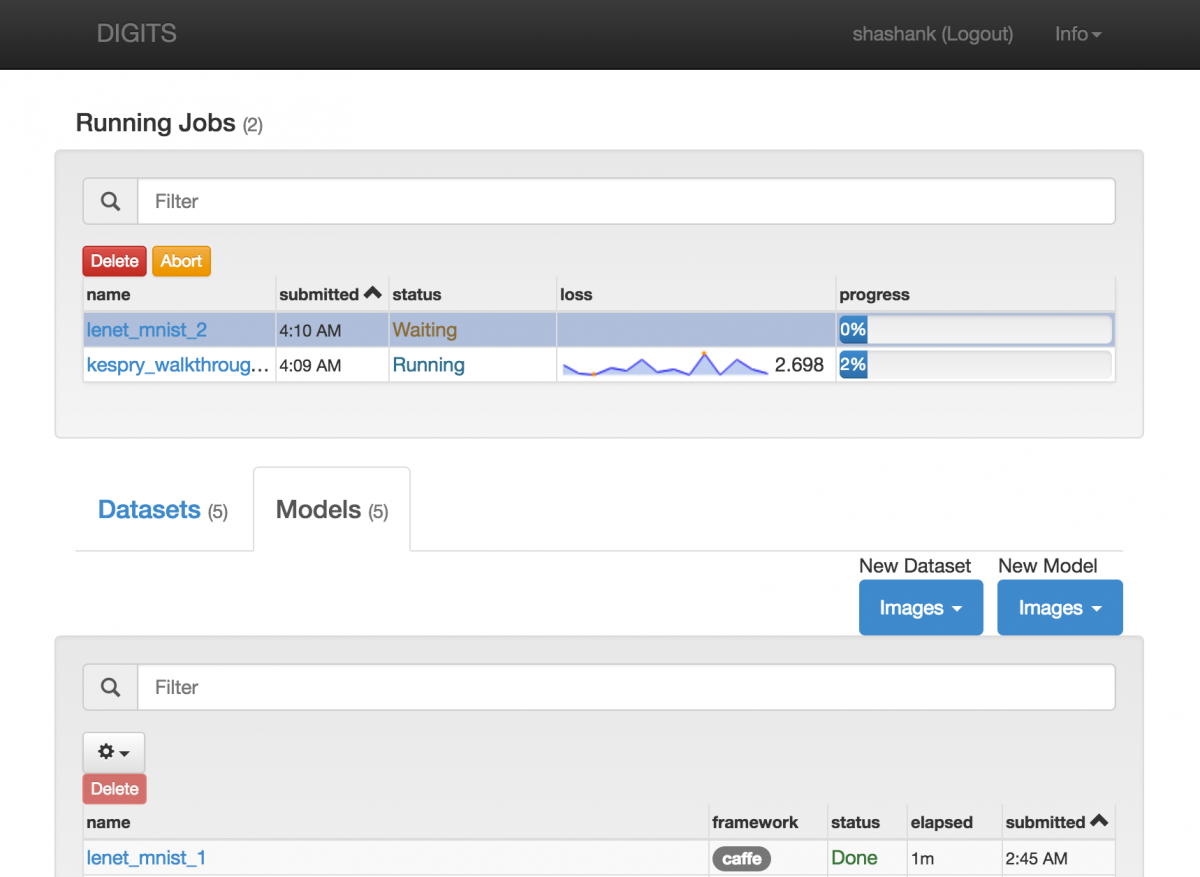
\includegraphics[width=\textwidth]{digits.png}
	\caption{An example of DIGITS' user interface}
	\label{fig:digits}
\end{figure}
\FloatBarrier

Due to these limitations, we aim to design BK.Synapse as a distributed training framework with little to no development overhead. Users should be able to train networks on multiple nodes with ease, while making minimal modifications to their existing codebases. With this in mind, we also target the more user-friendly PyTorch as the primary deep learning backend, with planned support for Keras and TensorFlow in the future. Table \ref{tab:digits_compare} shows a detailed comparison between BK.Synapse and DIGITS.

\begin{table}[]
\centering
\begin{tabu} to \textwidth {|l|X[c]|X[c]|}
    \hline
    \multicolumn{1}{|c|}{\textbf{Feature}} & \textbf{DIGITS} & \textbf{BK.Synapse} \\ \hline
    Single-node multi-GPU support & \cmark & \cmark \\ \hline
    Job monitoring \& management & \cmark & \cmark \\ \hline
    Open source & \cmark & \cmark \\ \hline
    Multiple node support & \xmark & \cmark \\ \hline
    Arbitrary models and datasets & \xmark & \cmark \\ \hline
    Data visualization & \cmark & \xmark \\ \hline
    Model visualization & \cmark & Partial (via Tensorboard) \\ \hline
    Backends & Caffe, TensorFlow, LuaTorch & PyTorch, Keras (planned), TensorFlow (planned) \\ \hline
\end{tabu}
\caption{Feature comparison between DIGITS and BK.Synapse}
\label{tab:digits_compare}
\end{table}

Aside from DIGITS, we also take note of other similar tools in the domain, namely DeepCognition\footnote{\href{https://deepcognition.ai/}{https://deepcognition.ai/}}, Google Colaboratory\footnote{\href{https://colab.research.google.com/}{https://colab.research.google.com/}}, etc,...

We shall describe BK.Synapse's design and technical implementation in the following section.

\subsection{System Description}
BK.Synapse is open source and hosted at \href{https://github.com/lanPN85/BK.Synapse}{https://github.com/lanPN85/BK.Synapse}.

\subsubsection{Core Concepts}
There are 4 core concepts that define the user's workflow in BK.Synapse (Figure \ref{fig:workflow}):
\begin{enumerate}
    \item Datasets: A dataset is a collection of arbitrary files used for training (eg. images, text files,...). There is no pre-defined format, and users can simply compress their existing data and upload to the server.
    \item Models: A model contains the code for the user's custom network. In order to facilitate dynamic loading during runtime, this code needs to adhere to a simple interface that will be described in later sections.
    \item Data loaders: A data loader is the glue component that connects a dataset and a model. Conceptually, data loaders are the same as PyTorch's Dataset or Keras' Sequence. They define how data from datasets should be loaded and transformed in order to be fed into models.
    \item Jobs: A job tie the above components together to create a complete training pipeline. It also specifies many hyperparameters for training (eg. learning rate, batch size,...) and the nodes to be used for the training process.
\end{enumerate}

\begin{figure}[htp]
	\centering
	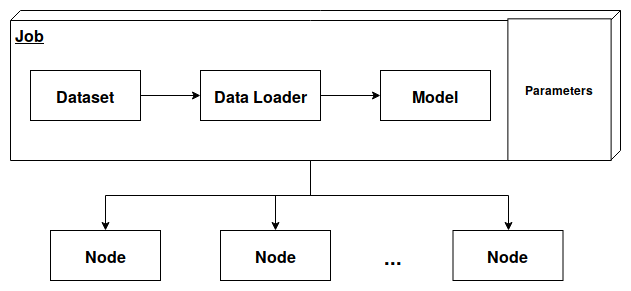
\includegraphics[width=0.6\textwidth]{workflow.png}
	\caption{BK.Synapse' core concepts and workflow}
	\label{fig:architecture}
\end{figure}
\FloatBarrier

\subsubsection{Architecture}
At a high level, BK.Synapse consists of 4 primary components (Figure \ref{fig:architecture}): the API server, worker nodes, data store, and the web application.

\begin{figure}[htp]
	\centering
	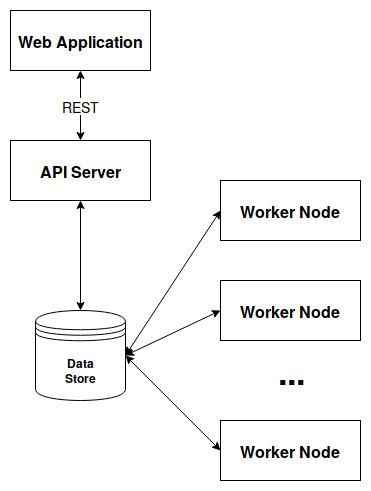
\includegraphics[width=0.65\textwidth]{architecture.png}
	\caption{BK.Synapse's high-level architecture}
	\label{fig:architecture}
\end{figure}

The system is designed in a client-server pattern, with loosely coupled components that can be deployed separately. The deployment environment should have high availability (ie. nodes should not fail or shutdown regularly) and trusted.

The API server exposes an application programming interface via HTTP REST\footnote{Representational State Transfer}. Clients can use standard HTTP requests from any supported language to access the system. The server is implemented with the Flask \cite{Grinberg:2014:FWD:2621997} framework.

Worker nodes handle the bulk of calculations during training. Each node runs a background process called the node daemon, collecting hardware status and notifying BK.Synapse of the node's availability.

The data store (or root folder) is used as the shared data space between the API server and worker nodes. It points to a folder that is accessible from all nodes within the system, and contains all user-uploaded data as well as additional metadata. Several mechanisms can be employed to create the data store, namely:
\begin{itemize}
    \item Using filesystem mount: The data store is created on one node, then mounted throughout the network using Linux's NFS or SMBD protocol. This provides good guarantees in terms of writes, however there may be overhead during training when data files need to be continually read.
    \item Using object store mount: Cloud object stores such as Amazon S3 or Minio provide utilities that allows mounting onto a folder. This can be significantly less trivial to setup compared to the first option, however it can perform much faster depending on the object store implementation.
\end{itemize}

The primary reason to use a native file folder as data store, as opposed to an object store or database is due to accessiblity. As stated, BK.Synapse aims to be simple and user-friendly, and thus should expose a simple folder structure to users instead of a complex data management system. With our setup, users can reuse their data loading logic directly into their BK.Synapse code.

Finally, the web application is a client that uses the BK.Synapse API, providing users with access to the system via a graphical interface (Figure \ref{fig:bks_example_1}). It also includes documentations and various examples of using BK.Synapse. The application is built using the Vue\footnote{\href{https://vuejs.org/}{https://vuejs.org/}} framework.

\begin{figure}[htp]
	\centering
	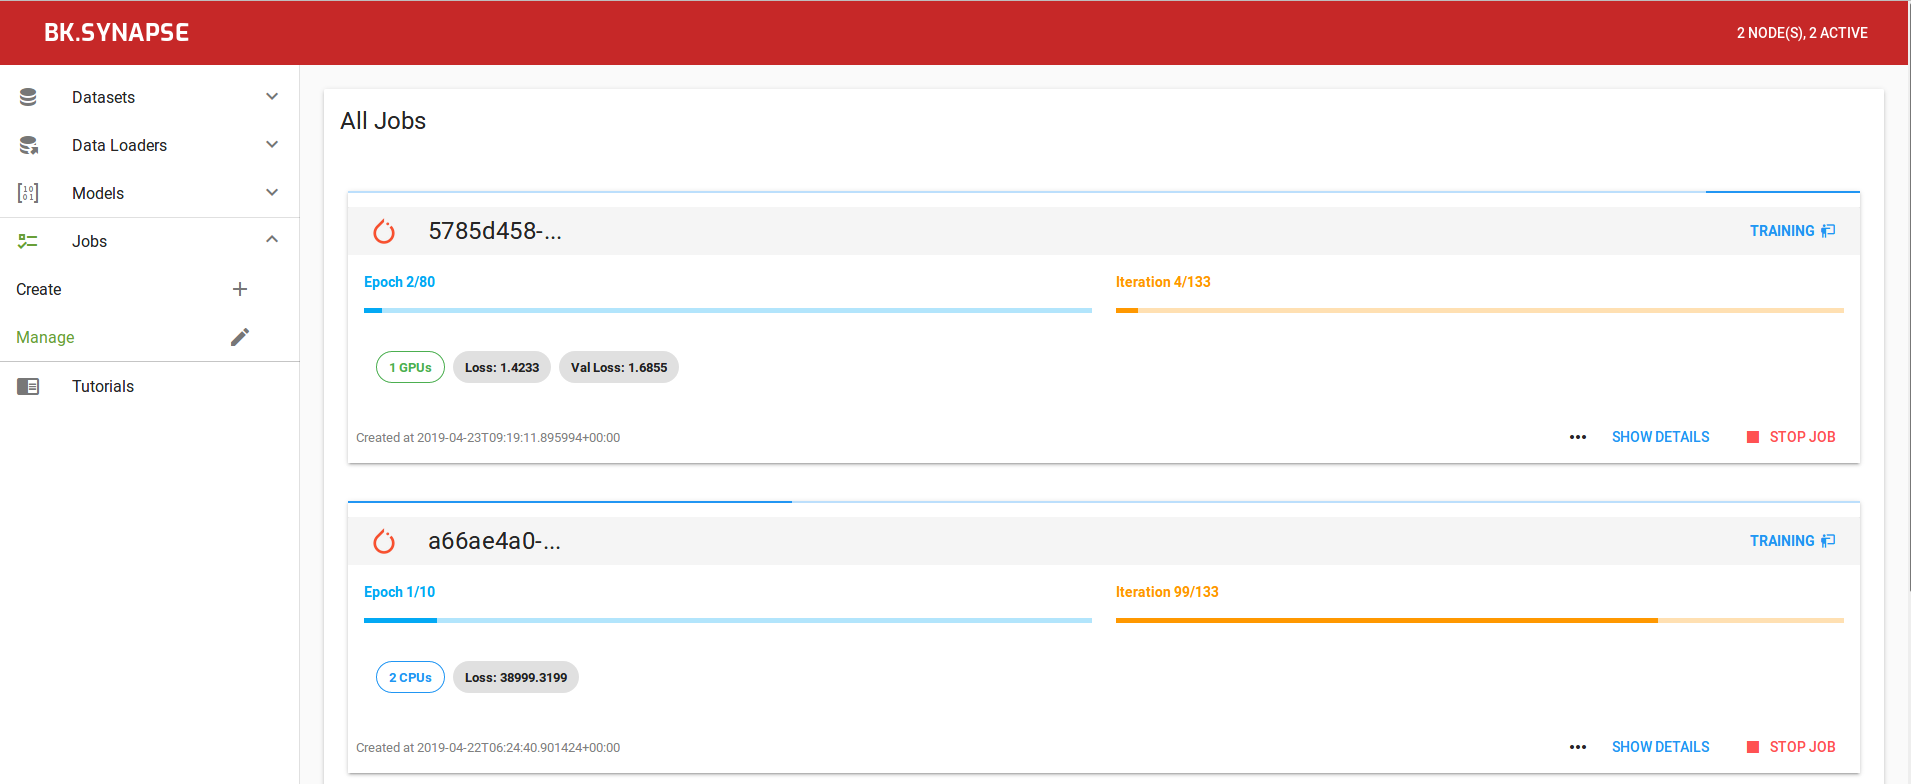
\includegraphics[width=\textwidth]{bks_example_1.png}
	\caption{The BK.Synapse web application}
	\label{fig:bks_example_1}
\end{figure}

\subsubsection{Dynamic Code Loading}

The core BK.Synapse runtime is capable of embedding user-defined classes and functions across multiple files/packages into the training procedure. This requires the user to define entrypoints that the runtime can detect. These include:
\begin{itemize}
    \item A file named \lstinline{bks_model.py}, containing the class \lstinline{UserModel} to define a model. \lstinline{UserModel} must implement a \lstinline{loss()} method that defines the loss function used in training. Optionally, if a \lstinline{metrics()} method is defined, then it is used to calculate additional metrics (eg. accuracy). For PyTorch models, \lstinline{UserModel} must subclass \lstinline{Module}.
    \item A file named \lstinline{bks_dataset.py}, containing the class \lstinline{UserDataset} and (optionally) \lstinline{UserValDataset}, which define the loading logic for a data loader. PyTorch-compatible loaders need to subclass PyTorch's \lstinline{Dataset} class.
\end{itemize}

These interfaces are meant to wrap around existing code using inheritance, thus preserving their original behavior and facilitate testing, while still conforming to BK.Synapse's specifications. Simpler models and loaders can simply be written directly into the given class.

\begin{lstlisting}[caption={An example UserModel wrapped around a simple CNN}]
import torch
import torch.nn as nn
import torch.nn.functional as F

class Net(nn.Module):
# ConvNet with 2 convolution blocks followed by dropout 
# and 2 fully connected layers
    def __init__(self):
        super(Net, self).__init__()
        self.conv1 = nn.Conv2d(1, 10, kernel_size=5)
        self.conv2 = nn.Conv2d(10, 20, kernel_size=5)
        self.conv2_drop = nn.Dropout2d()
        self.fc1 = nn.Linear(320, 50)
        self.fc2 = nn.Linear(50, 10)

    def forward(self, x):
        x = F.relu(F.max_pool2d(self.conv1(x), 2))
        x = F.relu(F.max_pool2d(self.conv2_drop(self.conv2(x)), 2))
        x = x.view(-1, 320)
        x = F.relu(self.fc1(x))
        x = F.dropout(x, training=self.training)
        x = self.fc2(x)
        return x

class UserModel(Net):
    def loss(self, output, target):
        return F.cross_entropy(output, target, reduction='mean')

    def metrics(self, output, target):
        preds = torch.argmax(output, dim=1)
        total = preds.shape[-1]
        correct = (preds == target).float()
        acc = torch.sum(correct) / total
        return {
            'accuracy': acc.item()
        }
\end{lstlisting}

The mechanics for embedding user code is relatively simple, and is partially based on DIGIT's method for loading TensorFlow models. We use Python's built-in \lstinline{exec()} function, which can execute a string as Python code within the current environment. A major difference in our implementation is allowing relative imports from within the model directory. Since actual projects would have their code split into multiple files, this is a critical feature to ensure ease of use. We accomplish this by manipulating Python's path object (\lstinline{sys.path}). The Python path is a list of filesystem paths that informs the interpreter where to look for modules. By inserting the source code root path to Python's path, we can emulate the user's environment and allow relative package loading. Once the neccessary modules are loaded, the injected path is removed to avoid pollution and/or conflict (Figure \ref{fig:codeload}).

\begin{figure}[htp]
	\centering
	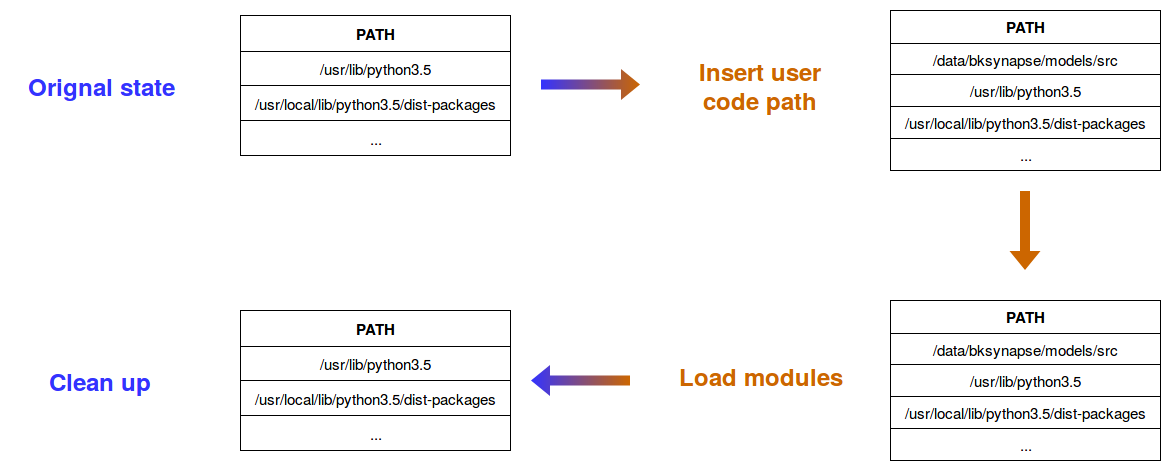
\includegraphics[width=0.95\textwidth]{codeload.png}
	\caption{Dynamic code loading procedure}
	\label{fig:codeload}
\end{figure}

\subsubsection{Parallelization Techniques}
BK.Synapse's key feature is being able to scale easily across multiple machines. The infrastructure layer supports this by keeping track of node IPs using node daemons, making it easy to add new nodes or detect failures. The actual parallel execution is implemented with Horovod \cite{DBLP:journals/corr/abs-1802-05799} and MPI \cite{Forum:1994:MMI:898758}.

Horovod provides a set of utilities to leverage MPI and associated acceleration methods (eg. NCCL) to perform multi-node training:
\begin{itemize}
    \item An \lstinline{hvd.rank()} function that provides the process MPI rank, as well as \lstinline{hvd.local_rank()} to query local MPI rank.
    \item A \lstinline{DistributedSampler} for PyTorch that partitions datasets into non-colliding sets for each process rank.
    \item A ring allreduce implementation (\lstinline{hvd.allreduce()}) providing efficient value aggregation.
    \item A \lstinline{DistributedOptimizer} wrapper for PyTorch that allows networks to be updated over multiple nodes.
\end{itemize}

The training script is invoked using \lstinline{mpirun}, from a subprocess spawned by the API server when the start endpoint is called. The server collects the selected worker nodes' IPs and generate a command as follow:
\begin{lstlisting}[language=Bash]
mpirun --allow-run-as-root -bind-to none -map-by slot\\
    -mca plm_rsh_args "-p 17992" -mca pml ob1 -mca btl ^openib\\
    -mca btl_tcp_if_include 192.168.1.0/24  -x LD_LIBRARY_PATH\\
    -x PATH -x BKSYN_DATA_ROOT -v -np 2\\
    -H 192.168.1.2:1,192.168.1.8:1\\
    python /usr/bin/bksynapse/pytorch/train.py\\
        --job-id d20db7d2-2f22-4f86-bbc7-8e93c5239132
\end{lstlisting}

A lot of configuration is handled by BK.Synapse to ensure proper MPI communication between nodes, in regards to the \lstinline{-mca} options above.

We make use of the rank 0 node as the logger, periodically writing the job's status to the shared folder. Interrupts are handled using a special lock file (\lstinline{job.lock}) that gets checked at regular intervals.

For nodes with multiple GPUs, the default behavior is to use all those that are available, each getting its own MPI process. We use local rank to pin each process to its respective GPU.

\subsubsection{Deployment Model}
All components are packaged as Docker containers for ease of deployment. The only system dependency is the shared data store, which is subsequently mounted to the \lstinline{/data} folder within each container.

MPI requires a single port to be used for SSH connection across all machines. To avoid collision, we use the port 17992, and bind each container to the host machine's network stack.

For optimal performance, we have several deployment recommendations:
\begin{itemize}
    \item High-speed connections are preferred when setting up the node network(eg. InfiniBand). Note that this does not have to include the web server, since this is separate from the training runtime.
    \item Node GPUs should have the same or similar capabilities. Otherwise, GPU speed or memory would be capped at the job's lowest-tier GPU, leading to wasted resources.
\end{itemize}

\subsubsection{Security Concerns}
In its current state, BK.Synapse should only be deployed in a trusted, private environment. This is due to a number of security concerns, including:
\begin{itemize}
    \item No access control or authorization has been implemented. This is however an important feature that will eventually be added once the API is more stable.
    \item The use of \lstinline{exec()} can create many attack vectors. Since \lstinline{exec()} would execute any Python command, a malicious agent can freely inspect or modify the system. Even though Docker provides some level of isolation, attackers can still easily cripple nodes or retrieve secret data. These vulnerabilities can be patched by setting up less-privileged users, or blocking certain modules from loading.
\end{itemize}

Since it is somewhat out-of-scope, we will not go into detail on this topic.

\section{Case Study: RetinaNet for Text Region Detection}  \label{section:retinanet}
